\PassOptionsToPackage{table}{xcolor}
\documentclass[t]{beamer}

\usepackage{physics}       % Everything physics
\AtBeginDocument{\RenewCommandCopy\qty\SI}
\usepackage{mathtools}     % To make equations look neater, e.g. \mathclap
\usepackage{siunitx}       % To do units, e.g. \qty{15}{\GeV} = 15 GeV
\usepackage{caption}       % Caption stuff for figures
\usepackage{slashed}       % Feynman slash
\usepackage{bm}            % Add bolding for Greek letters
\usepackage{multirow}      % More customization with tables
\usepackage{minted}        % For code blocks (make sure frame has 'fragile' option)
\usepackage{tikz}          % Shapes and such
\usetikzlibrary{arrows,shapes}
\usetikzlibrary{calc}
\tikzstyle{every picture}+=[remember picture]
\everymath{\displaystyle}
\usepackage{tikz-feynman}  % Feynman diagrams
\usepackage{qcircuit}      % Quantum Circuits

% Font stuff for tt+bf
\usepackage[T1]{fontenc}
\usepackage{libertine}
\usepackage[scaled=0.85]{beramono}

%%%%%%%%%%%%%%
%% CAPTIONS %%
%%%%%%%%%%%%%%
% Makes captions smaller, not starting with "Figure: " and centered
\captionsetup{
	font=scriptsize,
	%labelformat=empty,
	justification=centering
}
% Numbers the captions, doesn't do anything if `labelformat=empty' is uncommented
\setbeamertemplate{caption}[numbered]

\usepackage{mdframed}
\surroundwithmdframed{minted}

%%%%%%%%%%%%%%%
%% CITATIONS %%
%%%%%%%%%%%%%%%
\usepackage[backend=biber, sorting=none]{biblatex}
% Cites all references in the bib file, regardless of if they're cited in the slides
\nocite{*}
% Smaller font for references slide
\AtBeginBibliography{\scriptsize}
% Path to references
\addbibresource{references.bib}
% Prints out arxiv number of citation
\NewDocumentCommand{\arxivcite}{m}{
    \citefield{#1}{eprint}
}

%%%%%%%%%%%%
%% SLIDES %%
%%%%%%%%%%%%
% Removes navigation symbols at bottom of slide
\beamertemplatenavigationsymbolsempty
% Theming of slides: https://deic.uab.cat/~iblanes/beamer_gallery/individual/Darmstadt-default-default.html
\mode<presentation>{
	\usetheme{Darmstadt}
	% \usecolortheme{seahorse}
	\usefonttheme{structuresmallcapsserif}
}
% Title font, tt+bf
\setbeamerfont{frametitle}{series=\tt\bfseries, parent=structure}

% Custom color theme
\definecolor{bgCan}{RGB}{248, 237, 235}
\definecolor{txtBG}{RGB}{225, 187, 128}
\definecolor{txt}{RGB}{53, 34, 8}
\definecolor{hlBG}{RGB}{252, 213, 206}
\definecolor{hlFG}{RGB}{128, 100, 67}
\definecolor{struc}{RGB}{252, 213, 206}
\definecolor{item}{RGB}{104, 86, 52}
\definecolor{subitem}{RGB}{123, 107, 67}
\definecolor{bib}{RGB}{26, 20, 35}
\definecolor{bibTitle}{RGB}{171, 132, 118}
\definecolor{captionName}{RGB}{61, 49, 74}

\setbeamercolor{title}{bg=txtBG, fg=txt}
\setbeamercolor{author}{fg=txt}
\setbeamercolor{institute}{fg=txt}
\setbeamercolor{date}{fg=txt}
\setbeamercolor{background canvas}{bg=bgCan}
\setbeamercolor{structure}{fg=struc}
\setbeamercolor{frametitle}{fg=hlFG, bg=hlBG}
\setbeamercolor{item}{fg=item}
\setbeamercolor{subitem}{fg=subitem}
\setbeamercolor{bibliography entry author}{fg=bib}
\setbeamercolor{bibliography entry title}{fg=bibTitle}
\setbeamercolor{bibliography entry note}{fg=bib}
\setbeamercolor{caption name}{fg=captionName}


% Custom headline
\setbeamertemplate{headline}{%
\leavevmode%
  \hbox{%
    \begin{beamercolorbox}[wd=\paperwidth,ht=3ex,dp=1.5ex]{palette quaternary}%
    \insertsectionnavigationhorizontal{\paperwidth}{\hskip0pt plus1fill}{\hskip0pt plus1fill}
    \end{beamercolorbox}%
  }
}
\setbeamerfont{headline}{size=\tiny}

% Defines sub/subsubitems for itemize. Use [] with: triangle, circle, square, or ball. Or use custom with {}
\setbeamertemplate{itemize items}[circle]
\setbeamertemplate{itemize subitem}{\scriptsize$\blacktriangleright$}
\setbeamertemplate{itemize subsubitem}[square]
\setbeamertemplate{enumerate items}[circle]
\setbeamertemplate{enumerate subitem}{\scriptsize$\blacktriangleright$}
\setbeamertemplate{enumerate subsubitem}[square]
% Footnotes without a number marker: https://tex.stackexchange.com/a/30723
\makeatletter
\def\blfootnote{\gdef\@thefnmark{}\@footnotetext}
\makeatother

%%%%%%%%%%%%
%% MACROS %%
%%%%%%%%%%%%
\NewDocumentCommand{\stitle}{m}{
    \underline{\textbf{#1}}

}
\NewDocumentCommand{\colTitle}{m}{
    \begin{center}
        \stitle{#1}
    \end{center}
}
\NewDocumentCommand{\colSep}{O{0.05}}{
    \vrule{}
    \hspace{#1\textwidth}
}
% Horizontal line
\newcommand\hcut[1][black]{\noindent\textcolor{#1}{\rule{\textwidth}{1pt}}}

%%%%%%%%%%
%% MISC %%
%%%%%%%%%%
% Title slide
\title{\textbf{Title of the talk:}}
\subtitle{\textbf{A really good talk}}
\author{
    Your Name\\
    \footnotesize University of College\\
    \vspace{2em}
    \begin{scriptsize}
    \textbf{In collaboration with}\\
    Person One,
	Person Three,
	Todd Todderson
    \end{scriptsize}
}
\date{\textbf{Conference, Month Year}}

\begin{document}
\begin{frame}[plain]
    \titlepage
\end{frame}

\section{Section One}
\begin{frame}{Check this out}
    \only<1,2>{
        \begin{columns}
            \begin{column}[t]{0.3\textwidth}
                \colTitle{Column title}
                \begin{itemize}
                    \item Just some stuff
                    \item One the left-hand side
                \end{itemize}
            \end{column}
            \only<1>{\textcolor{txt!30!white}}{
                \colSep
                \begin{column}[t]{0.4\textwidth}
                    \colTitle{Integral}
                    ayayay
                    can't do enuemrates or itemizes tho :(
                \end{column}
            }
        \end{columns}
    }
    \only<3>{
        Now we change it completely
    }
\end{frame}

\begin{frame}{More stuff}
    upper text
    \hcut[black!30!bgCan]

    and a horiztonal line that you can specify the color of
\end{frame}

\section{Section}
\begin{frame}[c]{another title}
    hello there\\
    Citing something on the arxiv: \arxivcite{test2}\cite{test2}
    \blfootnote{numberless footnote!}
\end{frame}


\begin{frame}{Are you happy\onslide<2>{ or sad?}}
    \only<1>{
        \vspace{1.5em}
        only slide 1!
    }
    \onslide<2>{
        \centering
        slide 2!
        \begin{tikzpicture}[overlay]
            \node (circ) at (-0.6, 0.1) {};
            \draw<2>[black, thick] (circ) circle[radius=8mm] {};
            \node<2> (txt) at (-4.2, 3.8) {};
            \node<2>[fill=bgCan!70!black, rounded corners=1mm, align=left] (txt) at (-1.2, -2) {hello there};
            \path<2>[->] (txt) edge [line width=2px, black, bend left] (circ);
        \end{tikzpicture}
    }
\end{frame}

\section{Section Two}
\begin{frame}[c, fragile]{How It Runs}
    \begin{minted}[fontsize=\scriptsize, linenos, autogobble]{python}
        from package import foo

		var = foo('some python code')
\end{minted}
\end{frame}

\begin{frame}{References}
    \printbibliography
\end{frame}
\end{document}
